\chapter{Microbolómetros y descripción de especificaciones}
Los arreglos de microbolómetros son detectores de infrarrojos ampliamente utilizados en aplicaciones de imágenes térmicas. Están formados por una matriz bidimensional de microbolómetros, que son diminutos resistores sensibles a la temperatura diseñados para captar la radiación infrarroja que emiten los objetos dentro del campo de visión del detector. Estos sensores están montados sobre un sustrato de silicio y generalmente se fabrican utilizando tecnología MEMS (sistemas electromecánicos). Los detectores de este tipo ofrecen una resolución espacial y sensibilidad bastante altas, lo que permite que las matrices detecten y diferencien con precisión objetos con mínimas variaciones de temperatura.


Una ventaja adicional es que no necesitan enfriamiento externo, lo que hace que los sistemas de imágenes térmicas sean mas portátiles, fáciles de operar y adecuados para una amplia gama de aplicaciones \cite{Fusetto2023}.


Este dispositivo opera mediante una corriente o voltaje de polarización controlada que atraviesa el detector mientras se monitorea el voltaje o corriente de salida. En este proceso, la energía radiante genera calor en el material, lo que altera la resistencia, sin interacción directa entre fotones y electrones.


El astrónomo S.P. Langley diseñó el primer bolómetro en 1880, utilizando platino ennegrecido como material absorbente y un puente de Wheatstone como circuito de detección. La tecnología moderna de bolómetros comenzó en la década de los 80's con los avances de Honeywell en óxido de vanadio (VOx) y de Texas Instruments en silicio amorfo (a-Si). Mucho de este desarrollo ocurrió bajo proyectos militares clasificados en Estados Unidos, por lo que la divulgación de esta información a la comunidad científica data desde 1992.


Es muy difícil tener una representación exacta de un microbolómetro, pero este se puede representar como un circuito divisor de voltaje (Figura \ref{fig:voltage_divider}). Si el circuito está abierto y no hay radiación presente, el microbolómetro se encontrará a temperatura ambiente $T_{0}$, si el circuito está cerrado, la corriente fluirá y la resistencia del microbolómetro, $R_{B}$, se calentará, esto provocará que la temperatura incremente a $T_{1}$. Si ahora la radiación cae sobre el microbolómetro, la temperatura cambiará en un factor de $\Delta T$. Esto causará una modificación en la resistencia del microbolómetro, lo que a su vez generará una variación en el voltaje ($V_{RL}$) a través de la resistencia de carga $R_{L}$ \cite{Rogalski}. 

            \begin{figure}[hbtp]
                \centering
                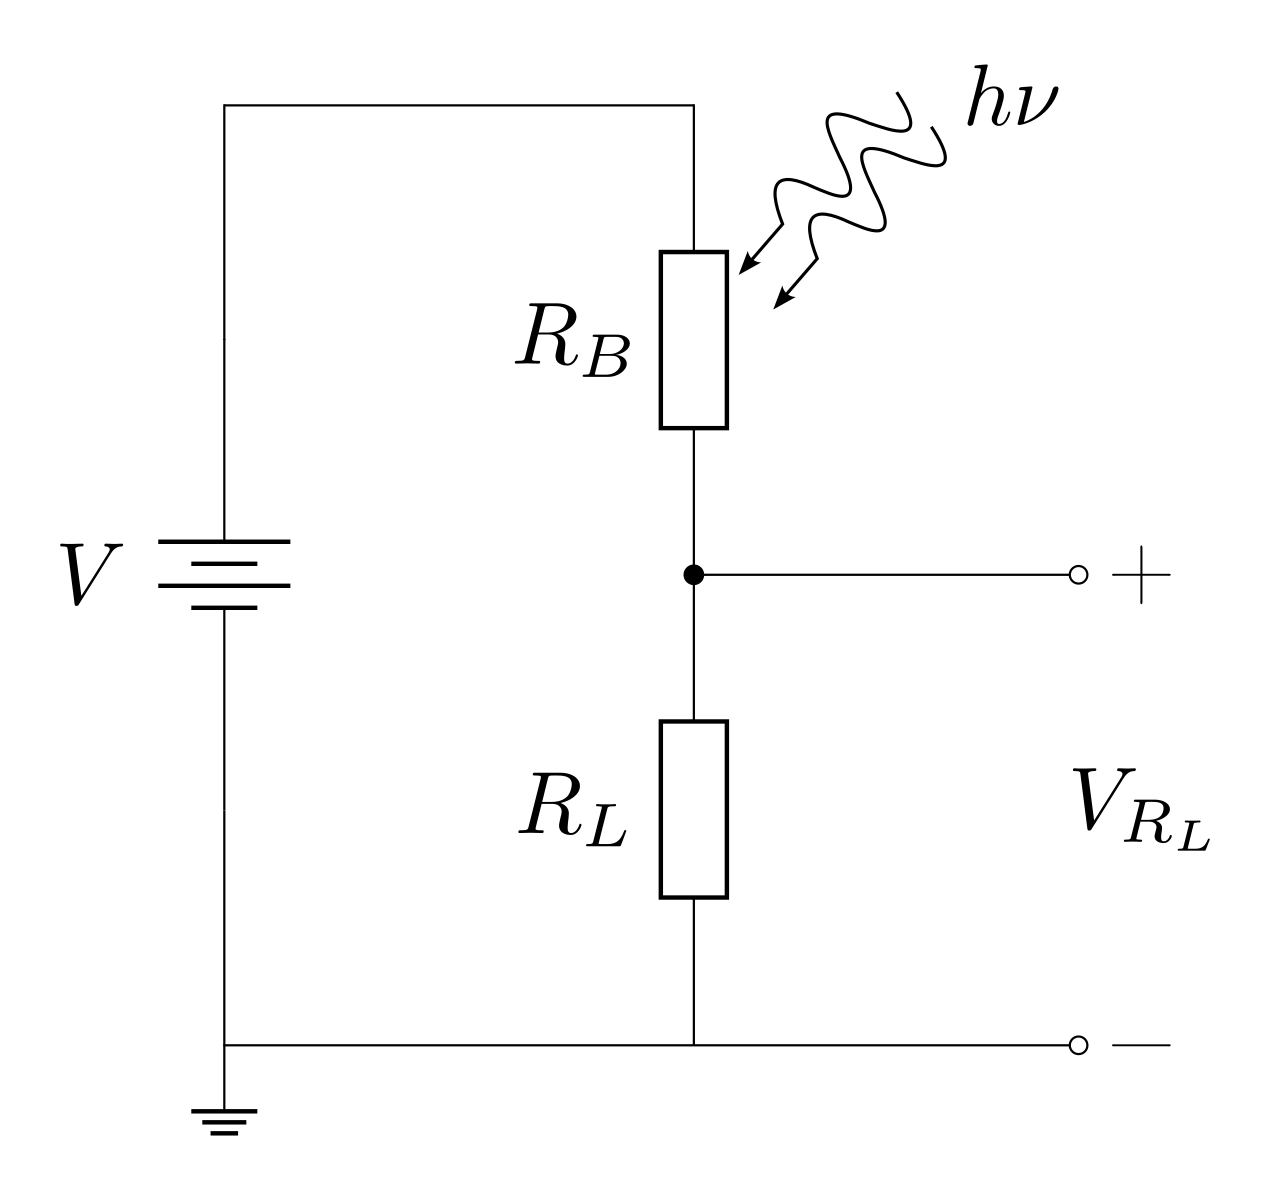
\includegraphics[width=0.4\textwidth]{voltage_divider}
                \caption{Representación de un microbolómetro como circuito eléctrico.}
                \label{fig:voltage_divider}
            \end{figure} 

\section{Diseño de un arreglo de microbolómetros}
El diseño de un microbolómetro generalmente incluye un material absorbedor y un material que funge como termómetro, lo que lleva a un incremento de la temperatura debido a la absorción de radiación infrarroja, provocando finalmente un cambio en la resistencia de sus elementos. La variación en la resistencia se transmite eléctricamente al circuito integrado de lectura (ROIC) para su posterior procesamiento. Para aumentar la sensibilidad, el termómetro se mantiene aislado térmicamente del sustrato del ROIC \cite{Bhan2009}.

El diagrama esquemático de la estructura típica de un microbolómetro se muestra en la Figura \ref{fig:ubol_sch}.
            \begin{figure}[hbtp]
                \centering
                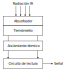
\includegraphics[width=0.4\textwidth]{ubol_sch}
                \caption{Diagrama esquemático de un microbolómetro.}
                \label{fig:ubol_sch}
            \end{figure}
\newpage
Un píxel en un arreglo de microbolómetros puede tener un área que varía entre $15\times 15\ \mu m^{2}$ y $55\times 55\ \mu m^{2}$. La estructura de un pixel, mostrada en la Figura \ref{fig:ubol_pixel}, generalmente es descrita como un \textit{puente}, el cual se trata de una membrana suspendida que incluye una capa absorbente para la radiación infrarroja y un elemento termosensible que transforma el cambio de temperatura de la membrana en una señal eléctrica de salida. El \textit{piso} de este \textit{puente} es un circuito de lectura unitario y las dos \textit{rampas} son brazos de soporte utilizados para la conexión eléctrica, estos ayudan a mejorar el aislamiento térmico \cite{Vincent}, \cite{Budzier}.

            \begin{figure}[hbtp]
                \centering
                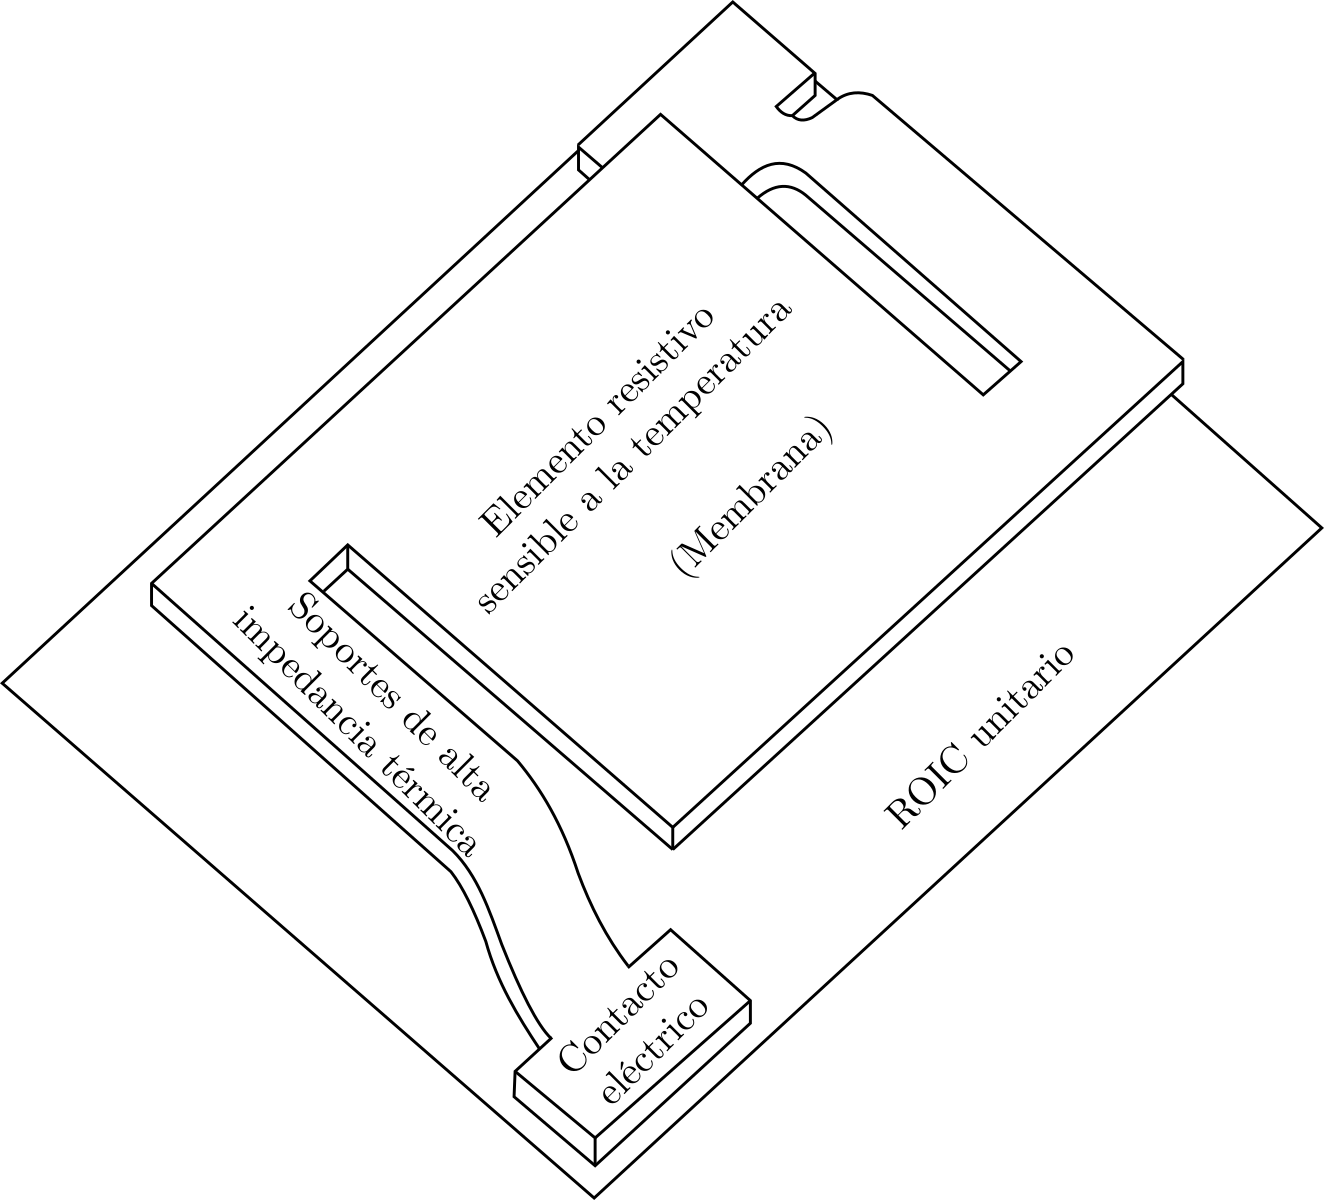
\includegraphics[width=0.8\textwidth]{ubol_pixel}
                \caption{Estructura de un pixel de un arreglo de microbolómetros.}
                \label{fig:ubol_pixel}
            \end{figure}

Para un microbolómetro es esencial contar con una temperatura estable, esto con la finalidad de tener una mejor detección de radiación infrarroja. El vacío provee un buen aislamiento térmico, debido a que la pérdida de calor por conducción o convección es mínima. Mientras más vacío se tenga en el envase del detector mejor será la eficiencia \cite{Lau2010}.
Generalmente el microbolómetro requiere una atmósfera de vacío menor a 1 Pa para aislar la transferencia de calor y mejorar su respuesta \cite{Liu2020}.


    \section{Propiedades}
    En esta sección se definirán algunas propiedades importantes que son utilizadas para caracterizar el desempeño de microbolómetros.
        \subsection{Responsividad}
        La responsividad ($R$) se refiere a la capacidad que tiene un detector de convertir radiación incidente en una señal eléctrica
        \begin{equation}
        R = \frac{se\tilde{n}al\ de\ salida}{radiaci\acute{o}n\ de\ entrada}
        \label{eq:Responsivity}
        \end{equation}
        
        Para los microbolómetros, generalmente la radiación de entrada se define en términos de flujo radiante ($\Phi_{S}$), el cual es el producto de la irradiancia ($E$) por el área del detector ($A_{d}$) y la señal de salida  puede ser voltaje ($V_{S}$) o corriente ($I_{S}$).
        \begin{equation}
        R = \frac{S}{\Phi_{S}}
        \label{eq:Responsividad}
        \end{equation}
        
        La responsividad de voltaje $R_{V}$ se define como:
        \begin{equation}
        R_{V} = \frac{V_{S}}{EA_{d}}\phantom{abc} [V/W]
        \label{eq:Rv}
        \end{equation}
        
        La responsividad de corriente es:
        \begin{equation}
        R_{I} = \frac{I_{S}}{EA_{d}}\phantom{abc} [A/W]
        \label{eq:Ri}
        \end{equation}
        
        La responsividad es un parámetro crucial para un detector, ayuda a anticipar la sensibilidad del circuito de medición necesario para observar la salida esperada o a decidir el nivel de ganancia del amplificador requerido para amplificar la señal adecuadamente \cite{Vincent}, \cite{Budzier}.
        
        \subsection{Diferencia de temperatura equivalente al ruido}
        La diferencia de temperatura equivalente al ruido (Noise Equivalent Temperature Difference - $NETD$), indica el cambio mínimo de temperatura que un microbolómetro puede detectar, reflejando su capacidad para distinguir pequeñas diferencias en la radiación térmica. Un valor de $NETD$ más bajo significa mayor sensibilidad térmica \cite{Jimenez}, \cite{Budzier}.


El NETD se define con la siguiente ecuación
        \begin{equation}
        NETD = \frac{4F^{2}V_{N}}{\tau_{0}A_{D}R(\Delta P/\Delta T)_{\lambda_{1}-\lambda_{2}}}
        \label{eq:NETD}
        \end{equation}
        
Donde $V_{N}$ es la tensión del ruido total; $F$ y $\tau_{0}$ son parámetros que tienen en cuenta la óptica del sistema; $(\Delta P/\Delta T)\lambda_{1}-\lambda_{2}$, es el cambio en la potencia emitida por unidad de superficie de un cuerpo negro dentro de una banda espectral específica, de $\lambda_{1}$ a $\lambda_{2}$, en función de la temperatura, y se expresa en Kelvin \cite{Fusetto2023}.
        
        \subsection{Detectividad}
        La detectividad ($D$) es un parámetro utilizado para comparar el desempeño entre distintos detectores con diferentes tamaños. Mientras más elevada sea la detectividad, mejor será el detector.
        
        La detectividad se calcula de la siguiente manera:
        \begin{equation}
        D = \frac{R_{V} \sqrt{A\Delta f}}{V_{N}}\phantom{abc} [cm\sqrt{Hz}/W]
        \label{eq:Detectivity}
        \end{equation}
        Donde $R_{V}$ es la responsividad de voltaje; $A$ es el área del detector; $\Delta F$ es el ancho de banda del ruido del detector y $V_{N}$ es ruido total del detector \cite{Vincent}, \cite{Jimenez}, \cite{Budzier}, \cite{Bhan2009}.
                
        \subsection{Conductancia térmica}
        La conductancia térmica ($G_{th}$) mide la facilidad con la que fluye el calor a través de un material. En el caso de un microbolómetro, cuantifica la velocidad a la que la energía térmica se transfiere del elemento detector a su entorno o al disipador de calor. La conductancia se puede obtener mediante la siguiente ecuación:
        
        \begin{equation}
        G_{th} = 2K\frac{A}{l}\phantom{abc} [W/K]
        \label{eq:Conductancia}
        \end{equation}
           
        Donde $K$ es el coeficiente de conductividad térmica del material de los brazos de soporte del microbolómetro; $A$ es el área transversal del brazo del detector; $l$ es la longitud del brazo \cite{BlancoMDA}, \cite{Jimenez} \cite{Bhan2009}.
        
        \subsection{Capacitancia térmica}
        La capacitancia térmica ($C_{th}$) determina cuánto calor puede almacenar el detector. Con la siguiente ecuación podemos calcularla.
        \begin{equation}
        C_{th} = c\rho v\phantom{abc} [J/K]
        \label{eq:Capacitancia}
        \end{equation}
         
        Donde $c$ es el calor específico del material; $\rho$ es la densidad del material con el que esté fabricado el pixel del microbolómetro; $v$ es el volumen de la membrana del microbolómetro \cite{BlancoMDA}, \cite{Jimenez} \cite{Bhan2009}.
        
        \subsection{Coeficiente de temperatura de la resistencia}
        El coeficiente de temperatura de la resistencia (Thermal Coefficient of Resistance - $TCR$) se define como la variación de la resistencia del microbolómetro ($R_{B}$) debido al cambio de temperatura:
        \begin{equation}
        \alpha_{B} = TCR =\frac{1}{R_{B}}\frac{dR_{B}}{dT_{S}}
        \label{eq:TCR}
        \end{equation}
        El cambio en la resistencia del microbolómetro en función de la temperatura depende de si el material es un metal o un semiconductor \cite{Budzier}, \cite{Wei2015}.  
               
        \subsection{Tiempo de respuesta térmico}
         El tiempo de respuesta térmico, $\tau_{th}$, se refiere al período que el sensor necesita para estabilizar la señal de corriente o voltaje que se mide tras un cambio en la temperatura. El cálculo de $\tau_{th}$ se obtiene con la siguiente ecuación \cite{Jimenez}.
        \begin{equation}
        \tau_{th} =\frac{C_{th}}{G_{th}}\phantom{abc} [s]
        \label{eq:Tth}
        \end{equation}          
Si la membrana es demasiado voluminosa, el detector responderá lentamente a los cambios de temperatura, mientras que una alta conductancia térmica permitirá una respuesta rápida. Por lo tanto, el diseño del microbolómetro implica un equilibrio entre la velocidad de respuesta y la sensibilidad \cite{Jimenez}.        
        

Todos estos parámetros pueden ser evaluados mediante la obtención de las curvas V-I del microbolómetro mientras opera en un entorno de vacío y está expuesto a iluminación infrarroja \cite{Hernandez2021}.

        
La clave para desarrollar microbolómetros altamente sensibles es tener un coeficiente de temperatura alto $\alpha$, una masa térmica muy baja $C_{th}$ y un excelente aislamiento térmico (baja conductancia térmica) $G_{th}$ \cite{Rogalski}.

\section{Circuitos de lectura para un microbolómetro}

Un circuito integrado de lectura (\textit{Readout Integrated Circuit} - ROIC), es un elemento esencial en los sistemas de imagen térmica. En los microbolómetros está integrado debajo de cada pixel. Los ROICs contienen todos los módulos necesarios para alimentar el microbolómetro, captar la variación de resistencia generada por la radiación infrarroja incidente, ajustarla y amplificarla para su posterior procesamiento \cite{BlancoMDA}, \cite{Budzier}, \cite{Fusetto2023}. El principal reto de un ROIC es disminuir el calentamiento del detector, para evitar información térmica errónea y que se incremente el riesgo de daño permanente \cite{Moreno2022}.


A continuación se presentan algunas topologías utilizadas como ROICs.

\subsection{Divisor resistivo} 
Esta topología está diseñada para medir la tensión en la salida de un divisor resistivo formado por un dispositivo de referencia y un microbolómetro, como se muestra en la Figura \ref{fig:divisor}. A medida que aumenta la radiación incidente en el microbolómetro, su resistencia disminuye proporcionalmente, lo que hace que la tensión de salida dependa de la radiación recibida por el sensor \cite{BlancoMDA}.
            \begin{figure}[hbtp]
                \centering
                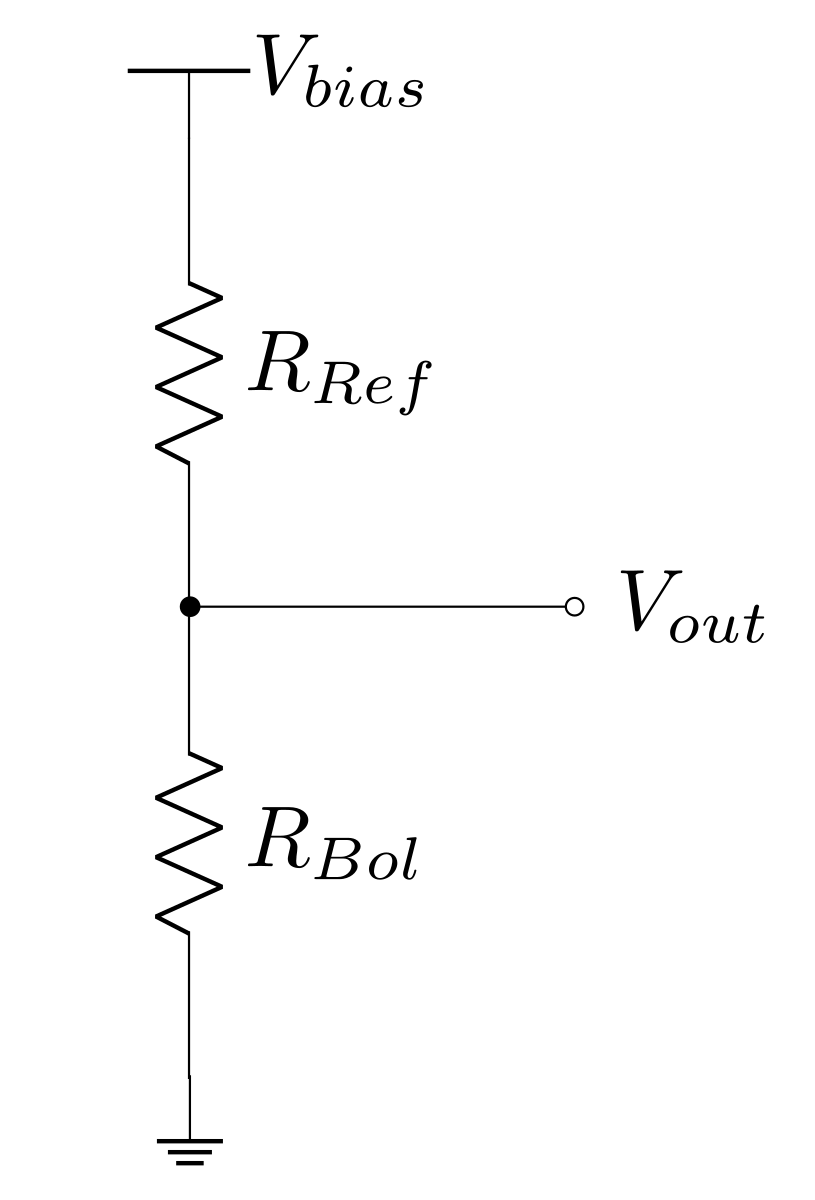
\includegraphics[width=0.3\textwidth]{divisor}
                \caption{Divisor resistivo.}
                \label{fig:divisor}
            \end{figure}

La tensión de salida se expresa con la siguiente ecuación:
        \begin{equation}
        V_{out} =\frac{V_{bias}}{R_{ref} + R_{bol}} = V_{0} - \Delta V_{out}
        \label{eq:Divisor}
        \end{equation} 
Donde:


$V_{0}$ - Valor de la tensión de salida en equilibrio térmico (sin radiación incidente)


$\Delta V_{out}$ - Valor de la disminución de la tensión de salida cuando hay radiación incidente sobre el microbolómetro.


Esta topología destaca por su simplicidad, bajo consumo de potencia, por atenuar el efecto de calentamiento en cada pixel del microbolómetro y por ocupar un área pequeña, no obstante, no tiene una restricción de frecuencia para el ruido, lo que impacta negativamente en la calidad de la señal de salida.

\subsection{Puente de Wheatstone}
Este tipo de ROIC obtiene la tensión de forma diferencial utilizando un puente Wheatstone, que está compuesto por dos ramas: una de referencia y otra que contiene el microbolómetro, como se muestra en la Figura \ref{fig:wheatstone}.

La parte superior de cada rama está compuesta por una resistencia de referencia, ambas con la misma magnitud resistiva ($R_{Ref_1} = R_{Ref_2}$). En la parte inferior de una de las ramas se encuentra el microbolómetro sensor, mientras que en la rama de referencia se ubica un microbolómetro aislado de la potencia incidente \cite{BlancoMDA}.
            \begin{figure}[hbtp]
                \centering
                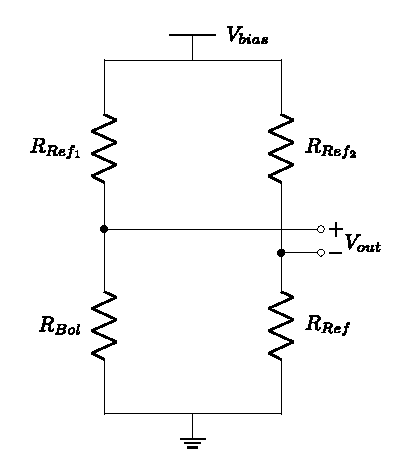
\includegraphics[width=0.45\textwidth]{wheatstone}
                \caption{Puente de Wheatstone.}
                \label{fig:wheatstone}
            \end{figure}

La tensión de salida es
        \begin{equation}
        V_{out} =\left(\frac{V_{bias}}{R_{Ref_1} + R_{Bol}}R_{Bol} - \frac{V_{bias}}{R_{Ref_2}+ R_{Ref}}R_{Ref} \right)
        \label{eq:Puente}
        \end{equation} 

La implementación del puente de Wheatstone como readout posibilita eliminar las contribuciones de voltaje en la salida causadas por el autocalentamiento debido a la polarización y las variaciones en los terminales de alimentación. No obstante, para alcanzar este objetivo, se incrementa tanto el área ocupada como el consumo de potencia.

\subsection{BCDI (Bolometer Current Direct Injection)}
Este circuito de lectura emplea un capacitor en el nodo de salida, el cual facilita el filtrado de frecuencias, lo que contribuye a disminuir el nivel de ruido. No obstante, la frecuencia de corte en la salida está determinada por el valor de la resistencia del microbolómetro. A medida que aumenta la potencia incidente, la resistencia disminuye y la frecuencia de corte se incrementa \cite{BlancoMDA}.
            \begin{figure}[hbtp]
                \centering
                \includegraphics[width=0.4\textwidth]{BCDI}
                \caption{Readout BCDI.}
                \label{fig:BCDI}
            \end{figure}

La tensión de salida se encuentra dada por la siguiente ecuación:
        \begin{equation}
        V_{out} =\frac{V_{Bias} R_{Bol}}{R_{Ref} (sR_{Bol} C+1) + R_{Bol}}
        \label{eq:bcdi}
        \end{equation}
La ventaja principal del BCDI, es su capacidad para limitar la frecuencia, lo que mejora la relación señal-ruido. No obstante, las contribuciones de voltaje en la salida debido al autocalentamiento y las variaciones en los terminales de polarización no se eliminan por completo.
\newpage
\subsection{CTIA (Capacitive Trans-Impedance Amplifier)}

Esta topología mostrada en la Figura \ref{fig:ctia}, presenta dos ventajas clave en comparación con otros circuitos de lectura. Primero, el uso de un amplificador operacional reduce considerablemente el ruido de la señal, lo que hace que esta topología sea especialmente adecuada para circuitos de lectura en detectores de alta resistividad sin refrigeración, así como en detectores de tipo diodo. La segunda ventaja importante es que se mantiene un nodo a una tensión constante, compartido entre la rama de referencia y la rama donde se encuentra el sensor, lo que asegura que el dispositivo de referencia esté polarizado de la misma manera que el microbolómetro \cite{BlancoMDA}.

            \begin{figure}[hbtp]
                \centering
                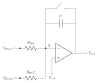
\includegraphics[width=0.55\textwidth]{ctia}
                \caption{Readout CTIA.}
                \label{fig:ctia}
            \end{figure}

Al mantener una tensión constante en el nodo X, se establece un nodo de tierra virtual que permite el flujo de la diferencia de corriente entre las dos ramas. Esta diferencia de corriente es integrada por el capacitor, convirtiéndose en una señal de tensión. Si la tensión $V_{Bias1}$ se reduce a $0V$, la tensión de salida se puede describir según lo indicado en la siguiente ecuación \cite{BlancoMDA}

        \begin{equation}
        V_{out} =\left(\frac{V_{Bias2}-V_{rst}}{R_{Ref}}-\frac{V_{rst}}{R_{Bol}}\right) \frac{1}{sC} \to \Delta V_{out} \approx i_{c}\frac{\Delta t}{C}
        \label{eq:ctia}
        \end{equation}
Este readout ofrece ventajas como la eliminación del efecto de calentamiento en la salida y la reducción del ruido gracias al uso de un capacitor que actúa como integrador de corriente. Sin embargo, su consumo de potencia es superior en comparación con las configuraciones anteriores, debido a la inclusión del amplificador, cuyo consumo de energía dependerá del diseño implementado.

\subsection{WBDA (Wheatstone Bridge Differential Amplifier)}
Este tipo de circuito de lectura se basa en el principio de un puente de Wheatstone, del cual se toma la tensión diferencial entre sus ramas, tal como se ilustra en la Figura \ref{fig:wbda}. Esta diferencia de tensión se amplifica mediante un amplificador de transconductancia o un amplificador de tensión. Finalmente, la señal de salida de la etapa de amplificación es integrada para reducir el ancho de banda y mejorar la relación señal/ruido.
            \begin{figure}[hbtp]
                \centering
                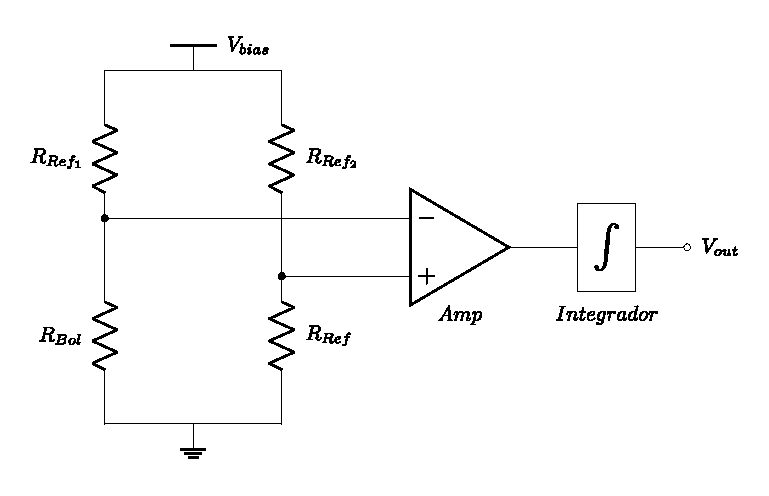
\includegraphics[width=0.8\textwidth]{wbda}
                \caption{Readout WBDA.}
                \label{fig:wbda}
            \end{figure}


En el caso donde la etapa de amplificación está compuesta por un amplificador de transconductancia y la etapa de integración por un capacitor, la tensión de salida se puede aproximar como

        \begin{equation}
        V_{out} = \frac{\frac{V_{Bias}}{R_{Ref}}}{1+\frac{R_{Ref}}{R_{0}}}\cdot (\Delta R)\cdot G_{m}\cdot \frac{1}{sC}
        \label{eq:wbda}
        \end{equation}
El rendimiento de este readout compensa eficazmente el efecto de calentamiento y limita la banda de frecuencia para reducir el ruido en la señal. No obstante, para lograr la compensación del calentamiento, se utiliza un puente de Wheatstone, lo que incrementa el área ocupada. Además, las etapas de amplificación y filtrado de la señal también contribuyen a un mayor consumo de potencia.        
\newpage
\subsection{CCBDI (Constant Current Buffered Direct Injection)}
Este método de readout se basa en medir la diferencia de voltajes entre un microbolómetro polarizado con una corriente $I_{0}$ y un voltaje de referencia generado por un amplificador de transconductancia. El diagrama del circuito se presenta en la Figura \ref{fig:ccbdi}.
            \begin{figure}[hbtp]
                \centering
                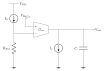
\includegraphics[width=0.6\textwidth]{ccbdi}
                \caption{Readout CCBDI.}
                \label{fig:ccbdi}
            \end{figure}

La diferencia de voltaje entre el voltaje aplicado del microbolómetro, $V_{Bol}$ y el voltaje de referencia del amplificador, $V_{Ref_{gm}}$, es convertida en corriente mediante el amplificador de transconductancia. En la etapa final, se incluye una corriente de referencia, $I_{s}$, cuya función es restar parte de la corriente amplificada; finalmente, un capacitor actúa como un integrador en la salida. Idealmente, el voltaje de salida de este circuito se describe mediante la ecuación que se muestra a continuación

        \begin{equation}
        V_{out} = \frac{G_{m}(V_{Bol}-V_{Ref_{gm}})-I_{s}}{sC}
        \label{eq:ccbdi}
        \end{equation}
Este readout reduce en su totalidad el ruido mediante la disminución del ancho de banda en frecuencia a expensas de un mayor consumo de energía y un aumento en el área ocupada.

\newpage
Los circuitos de lectura empleados para detectar señales de microbolómetros tienen como objetivo principal minimizar el ruido y reducir el calentamiento del detector, lo cual es esencial para preservar la precisión y sensibilidad del dispositivo. Sin embargo, existe un compromiso inherente en el diseño de estos circuitos: cuanto más efectivo sea el circuito en disminuir el ruido y los efectos térmicos, mayor será su consumo de potencia y el área ocupada en el chip. Este compromiso entre eficiencia en la reducción de ruido y optimización de recursos es un factor crucial en el diseño de sistemas de lectura para microbolómetros.          


En la siguiente tabla se muestra un resumen de las topologías mencionadas anteriormente.
            \begin{table}[hbtp]
                \caption{Topologías ROIC.}
                \begin{center}
                    \resizebox{1\linewidth}{!}{ 
                    \begin{NiceTabular}{|l|c|c|c|c| }
                        \CodeBefore
                        \Body
                        \hline
                        \textbf{Topología} & \textbf{Reducción de ruido} & \textbf{Reducción de calentamiento} & \textbf{Consumo de potencia} & \textbf{Área ocupada}\\
                        \hline
                        Divisor resistivo& &$\bullet$ &$\downarrow$ &$\downarrow$ \\
                        Puente de Wheatstone& &$\bullet$ &$\uparrow$ &$\uparrow$ \\
                        BCDI&$\bullet$& &$\downarrow$ &$\downarrow$ \\
                        CTIA&$\bullet$&$\bullet$& $\uparrow$ & $\uparrow$ \\
                        WBDA& $\bullet$ & $\bullet$ & $\uparrow$ & $\uparrow$ \\
                        CCBDI& $\bullet$ & &$\uparrow$ & $\uparrow$\\
                        \hline
                    \end{NiceTabular}
                    }
                \label{tab:Div_IR}
                \end{center}
            \end{table}
            
\newpage            
\section{Generación de imágenes infrarrojas con microbolómetros}            
La señal proveniente de los microbolómetros debe ser acondicionada y convertida a formato digital para su almacenamiento y procesamiento. Estos datos permiten crear una imagen térmica\cite{Moreno2022}.


El sistema para generar una imagen a partir de microbolómetros incluye los componentes mostrados en la Figura \ref{fig:sch_image_ubol}.

            \begin{figure}[hbtp]
                \centering
                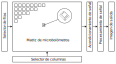
\includegraphics[width=0.9\textwidth]{sch_image_ubol}
                \caption{Esquema de formación de imágenes a partir de microbolómetros.}
                \label{fig:sch_image_ubol}
            \end{figure} 

El sistema para generar una imagen requiere una matriz de microbolómetros donde cada sensor cambia su resistencia según la potencia infrarroja recibida. Esta señal debe ser procesada por un circuito de lectura. El acceso y organización de cada señal se realiza mediante el direccionamiento de filas y columnas, que permite organizar las señales de los píxeles para formar la imagen final.


El proceso de formación de la imagen se puede resumir en \cite{BlancoMDA}, \cite{Hernandez2021}:
\begin{enumerate}
 \item Polarización de cada microbolómetro empleando un convertidor D/A.
 \item Direccionamiento y acceso a cada microbolómetro para acondicionar la señal mediante un circuito de lectura.
 \item Lectura de la señal proveniente del circuito de lectura por medio de un convertidor A/D.
 \item Recepción y captura de datos mediante software.
 \item Interpretación y procesamiento de datos para la generación de una imagen.
\end{enumerate}

Una tarjeta de adquisición de datos es responsable de direccionar cada píxel de la matriz de microbolómetros, controlando tanto los convertidores D/A y A/D. Además, recibe y envía los datos provenientes del circuito de lectura, facilitando su posterior procesamiento para generar la imagen infrarroja. Este componente es esencial para coordinar la transferencia de información y asegurar la correcta formación de la imagen \cite{Hernandez2021}.